\documentclass[a4paper,11pt]{article}
\usepackage[UTF8]{ctex}
\usepackage{pdfpages}
\usepackage{zh_CN-Adobefonts_external} 
\usepackage{geometry}
\usepackage{fancyhdr} 
\usepackage{minted} 
\usepackage[colorlinks,
linkcolor=black,CJKbookmarks,
]{hyperref}
\usepackage[T1]{fontenc}
\usepackage[utf8]{inputenc}
\setlength{\headheight}{15pt}
\pagestyle{fancy}
\fancyhf{}
\fancyhead[C]{ACM Templates by XTS}
\lfoot{}
\cfoot{\thepage}
\rfoot{}

\author{XTS}   
\title{ACM Templates}
\hyphenpenalty=500000
\tolerance=10
\geometry{a4paper,left=2cm,right=2cm,top=3cm,bottom=3cm}
\begin{document} 
\maketitle 
\newpage
\tableofcontents




\newpage
\section{图论} % 一级标题

\subsection{dijstra}
\inputminted[breaklines]{c++}{Graph/dijstra.cpp}

\subsection{倍增LCA}%三级标题
\inputminted[breaklines]{c++}{Graph/lca.cpp}

\subsection{树上路径交}
\inputminted[breaklines]{c++}{Graph/树上路径交.cpp}

\subsection{树链剖分}
\inputminted[breaklines]{c++}{Graph/树链剖分.cpp}

\subsection{点分治}
\inputminted[breaklines]{c++}{Graph/点分治.cpp}

\subsection{强连通分量}
\inputminted[breaklines]{c++}{Graph/scc.cpp}

\subsection{双连通分量}
\inputminted[breaklines]{c++}{Graph/bcc.cpp}

\subsection{仙人掌求环}
\inputminted[breaklines]{c++}{Graph/仙人掌求环.cpp}

%\twocolumn  分栏






\newpage
\section{字符串}

\subsection{回文树}
\inputminted[breaklines]{c++}{String/pam.cpp}

\subsection{广义后缀自动机}
\inputminted[breaklines]{c++}{String/sam.cpp}

\subsection{kmp}
\inputminted[breaklines]{c++}{String/kmp.cpp}


\newpage
\section{数据结构}











\newpage
\section{数学} % 一级标题

\subsection{带预处理BGSG}
\inputminted[breaklines]{c++}{Math/BGSG.cpp}

\subsection{十进制矩阵快速幂}
\inputminted[breaklines]{c++}{Math/快速幂.cpp}

\subsection{exlucas}
\inputminted[breaklines]{c++}{Math/exlucas.cpp}

\subsection{BM}
\inputminted[breaklines]{c++}{Math/BM.cpp}

\subsection{杜教筛}
\inputminted[breaklines]{c++}{Math/杜教筛.cpp}

\subsection{线性基}
\inputminted[breaklines]{c++}{Math/线性基.cpp}

\subsection{原根}
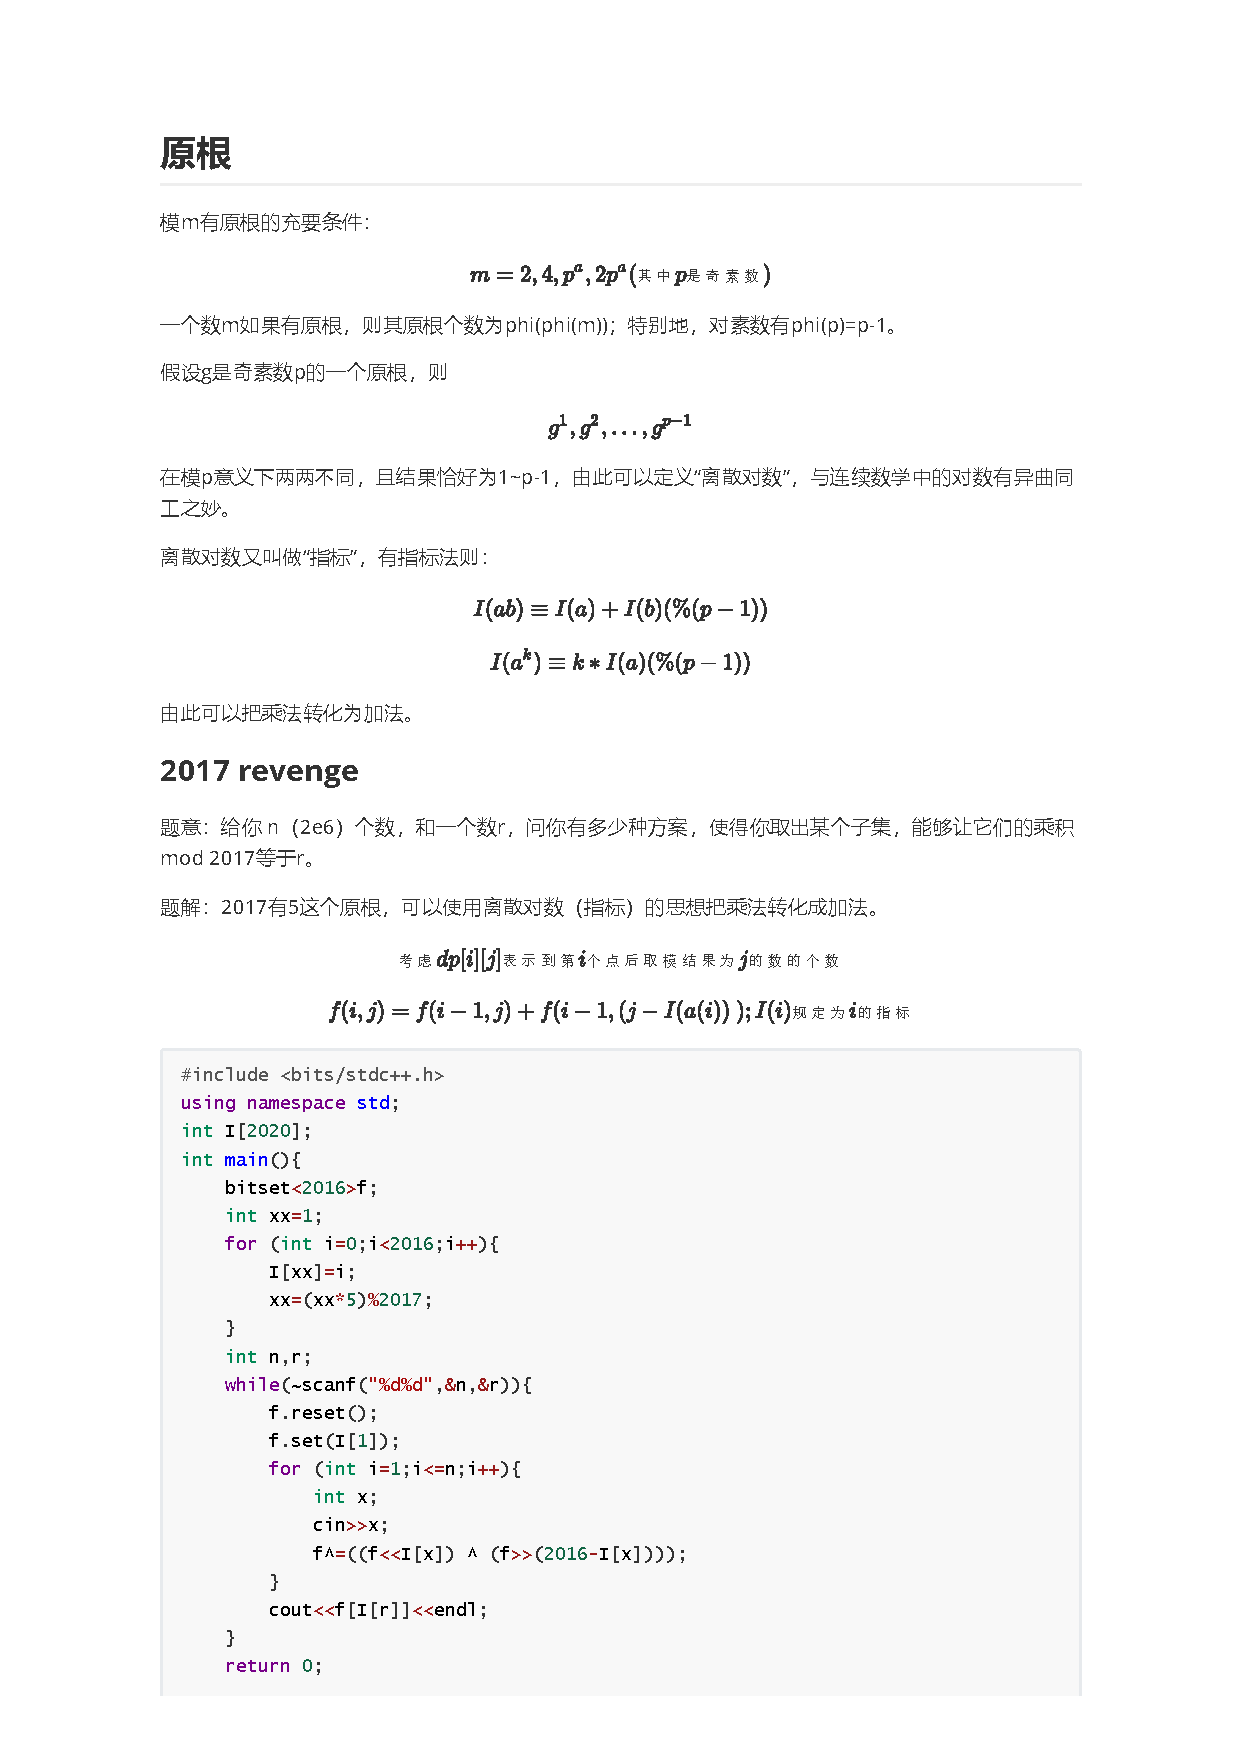
\includepdf[pages={1}]{Math/原根.pdf}

\subsection{欧拉降幂}
\inputminted[breaklines]{c++}{Math/欧拉降幂.cpp}

\subsection{拉格朗日插值}
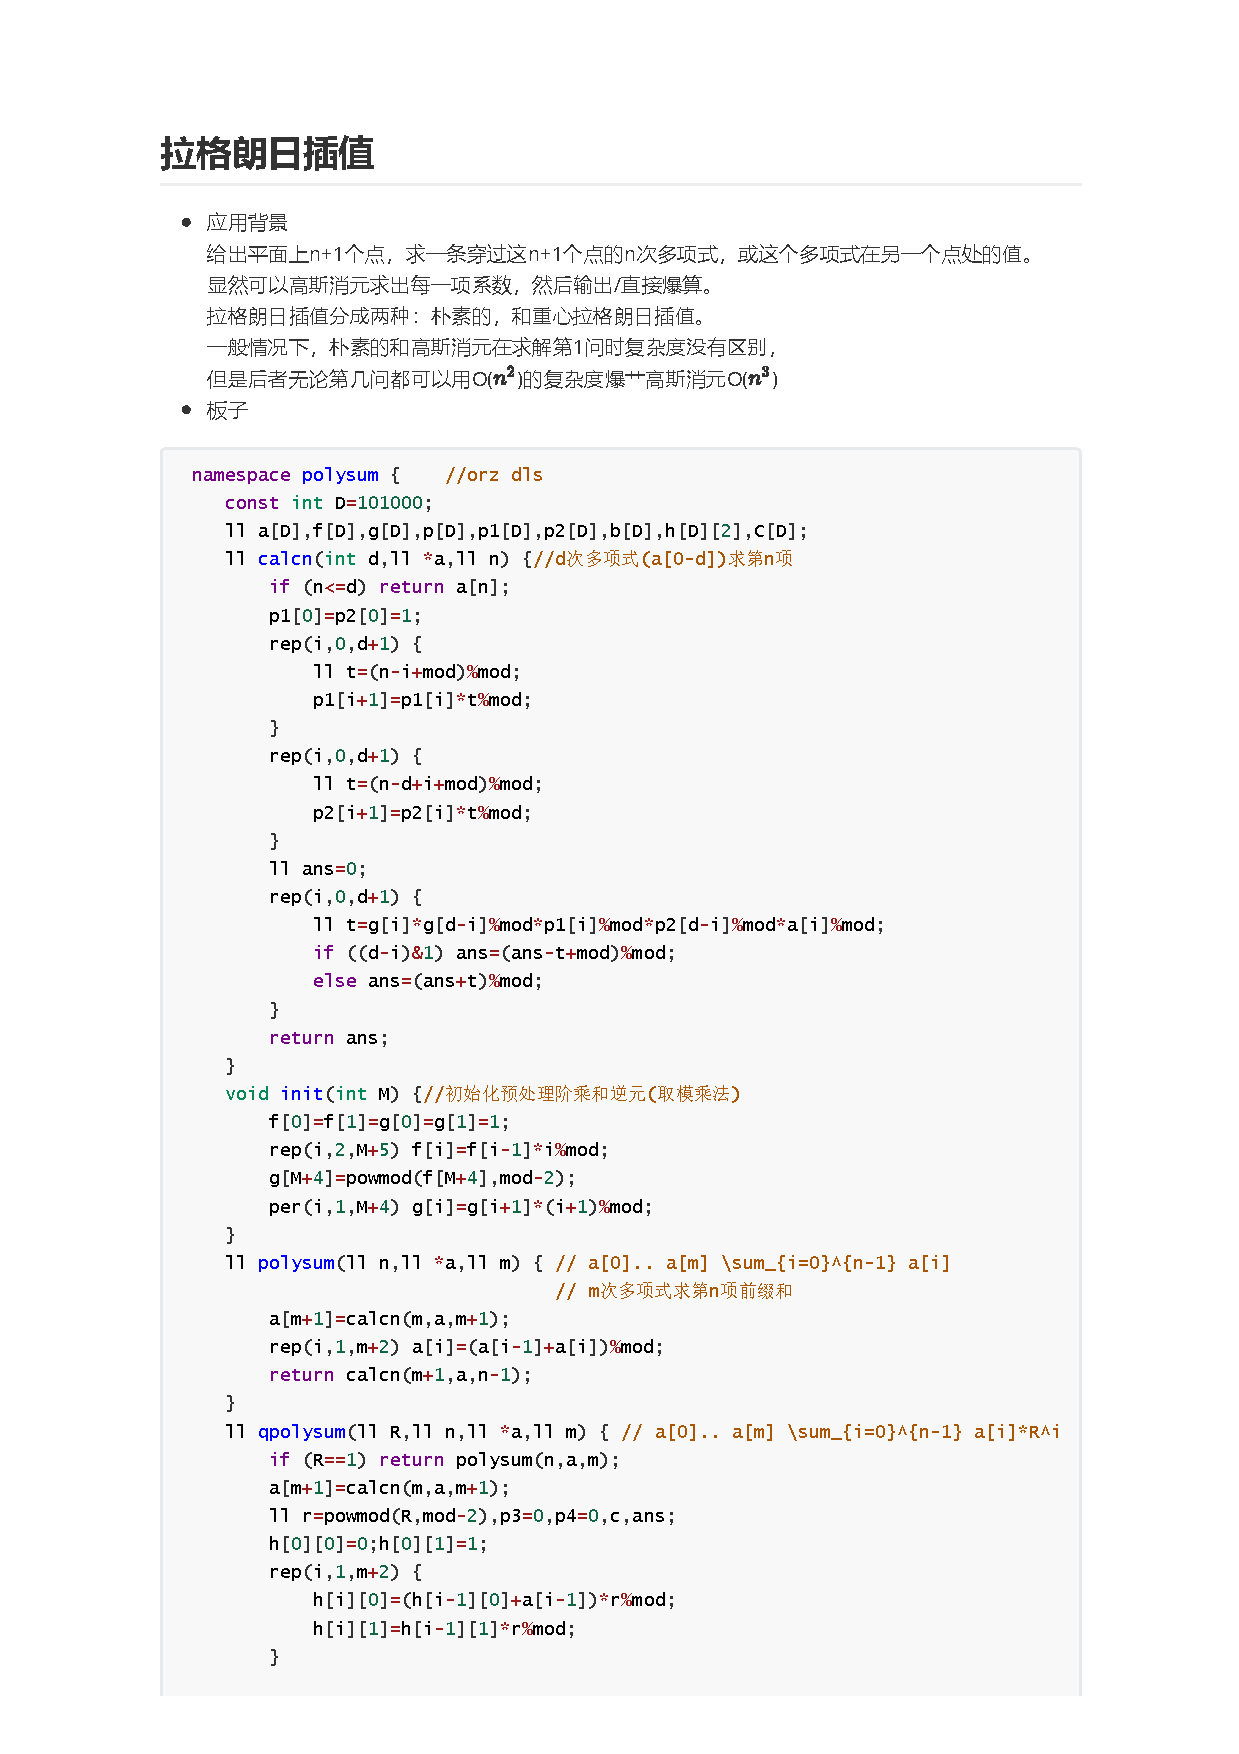
\includepdf[pages={1,2}]{Math/拉格朗日插值.pdf}

\subsection{伯努利数}
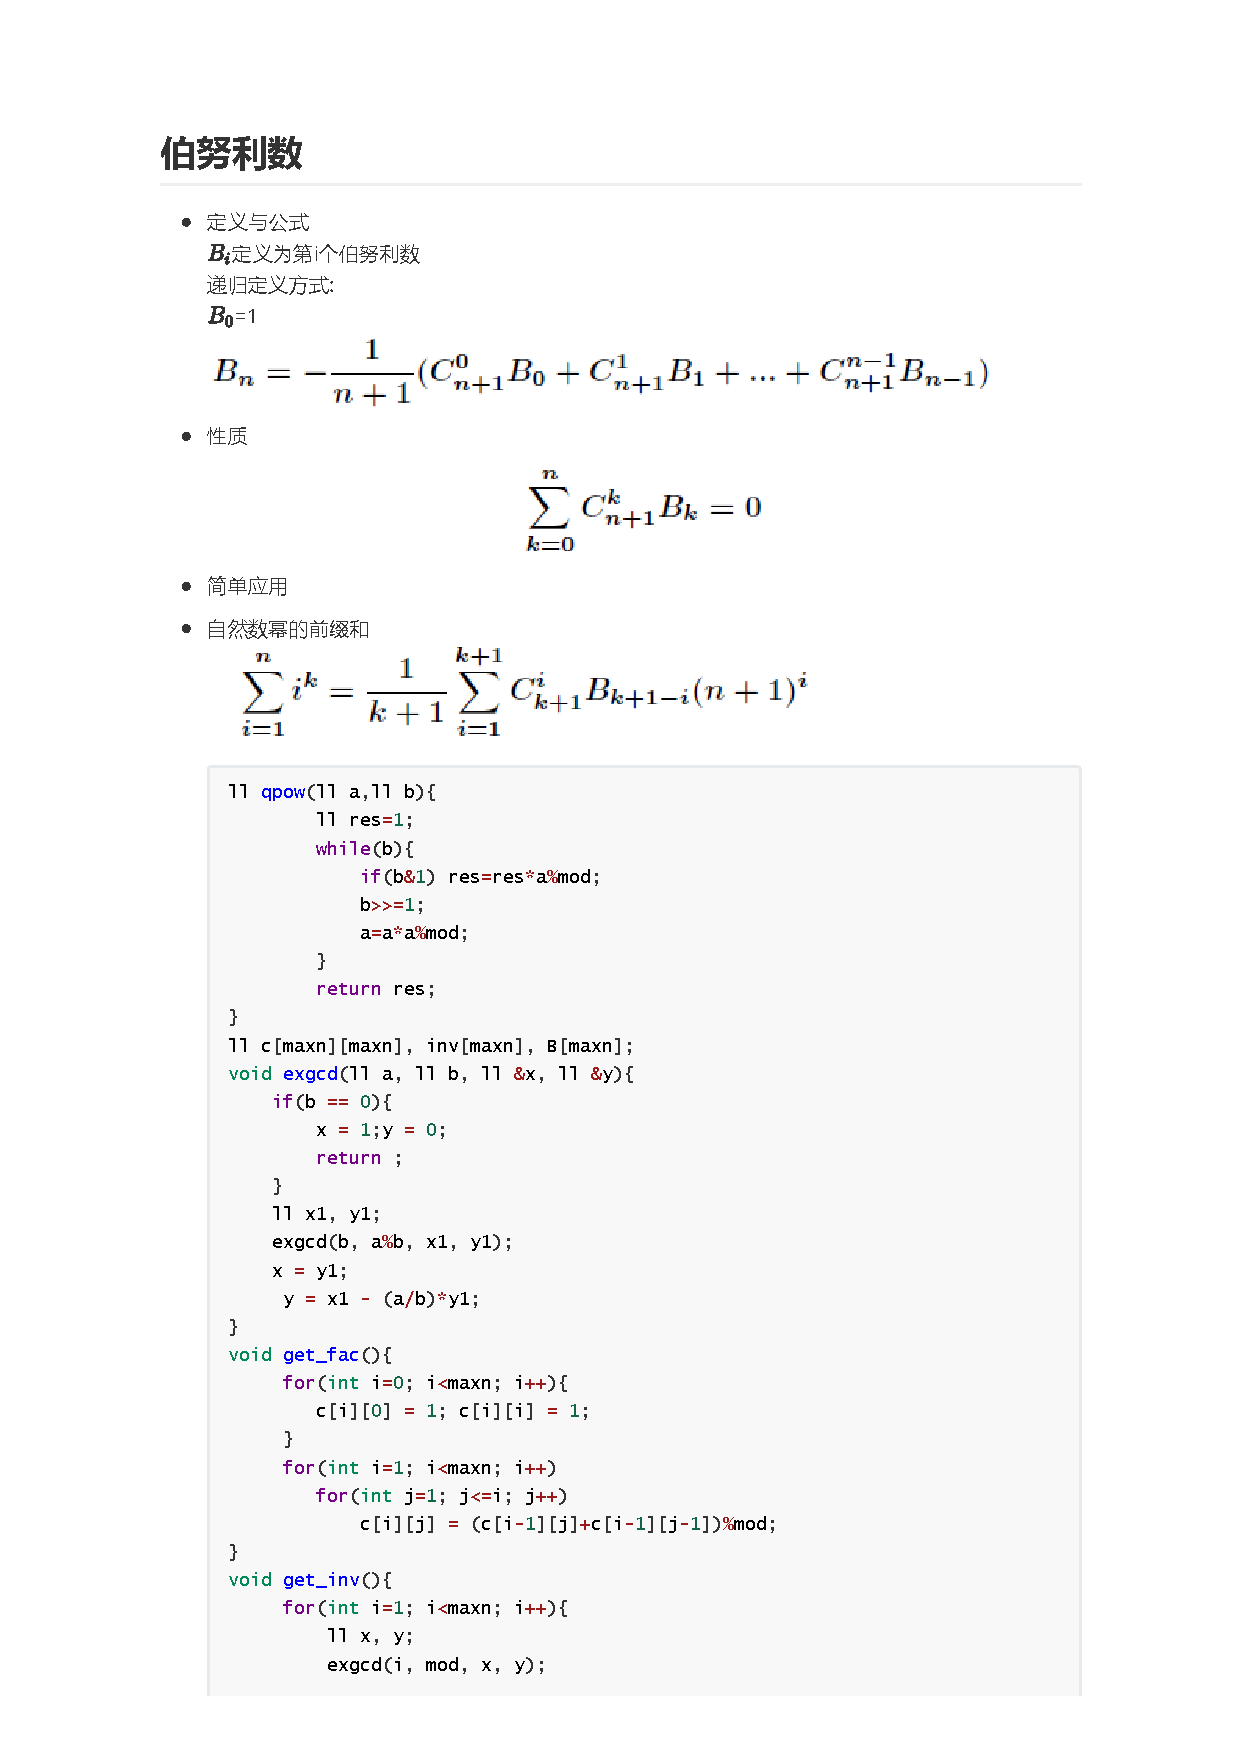
\includepdf[pages={1,2}]{Math/伯努利数.pdf}

\subsection{FFT&NTT&FWT}
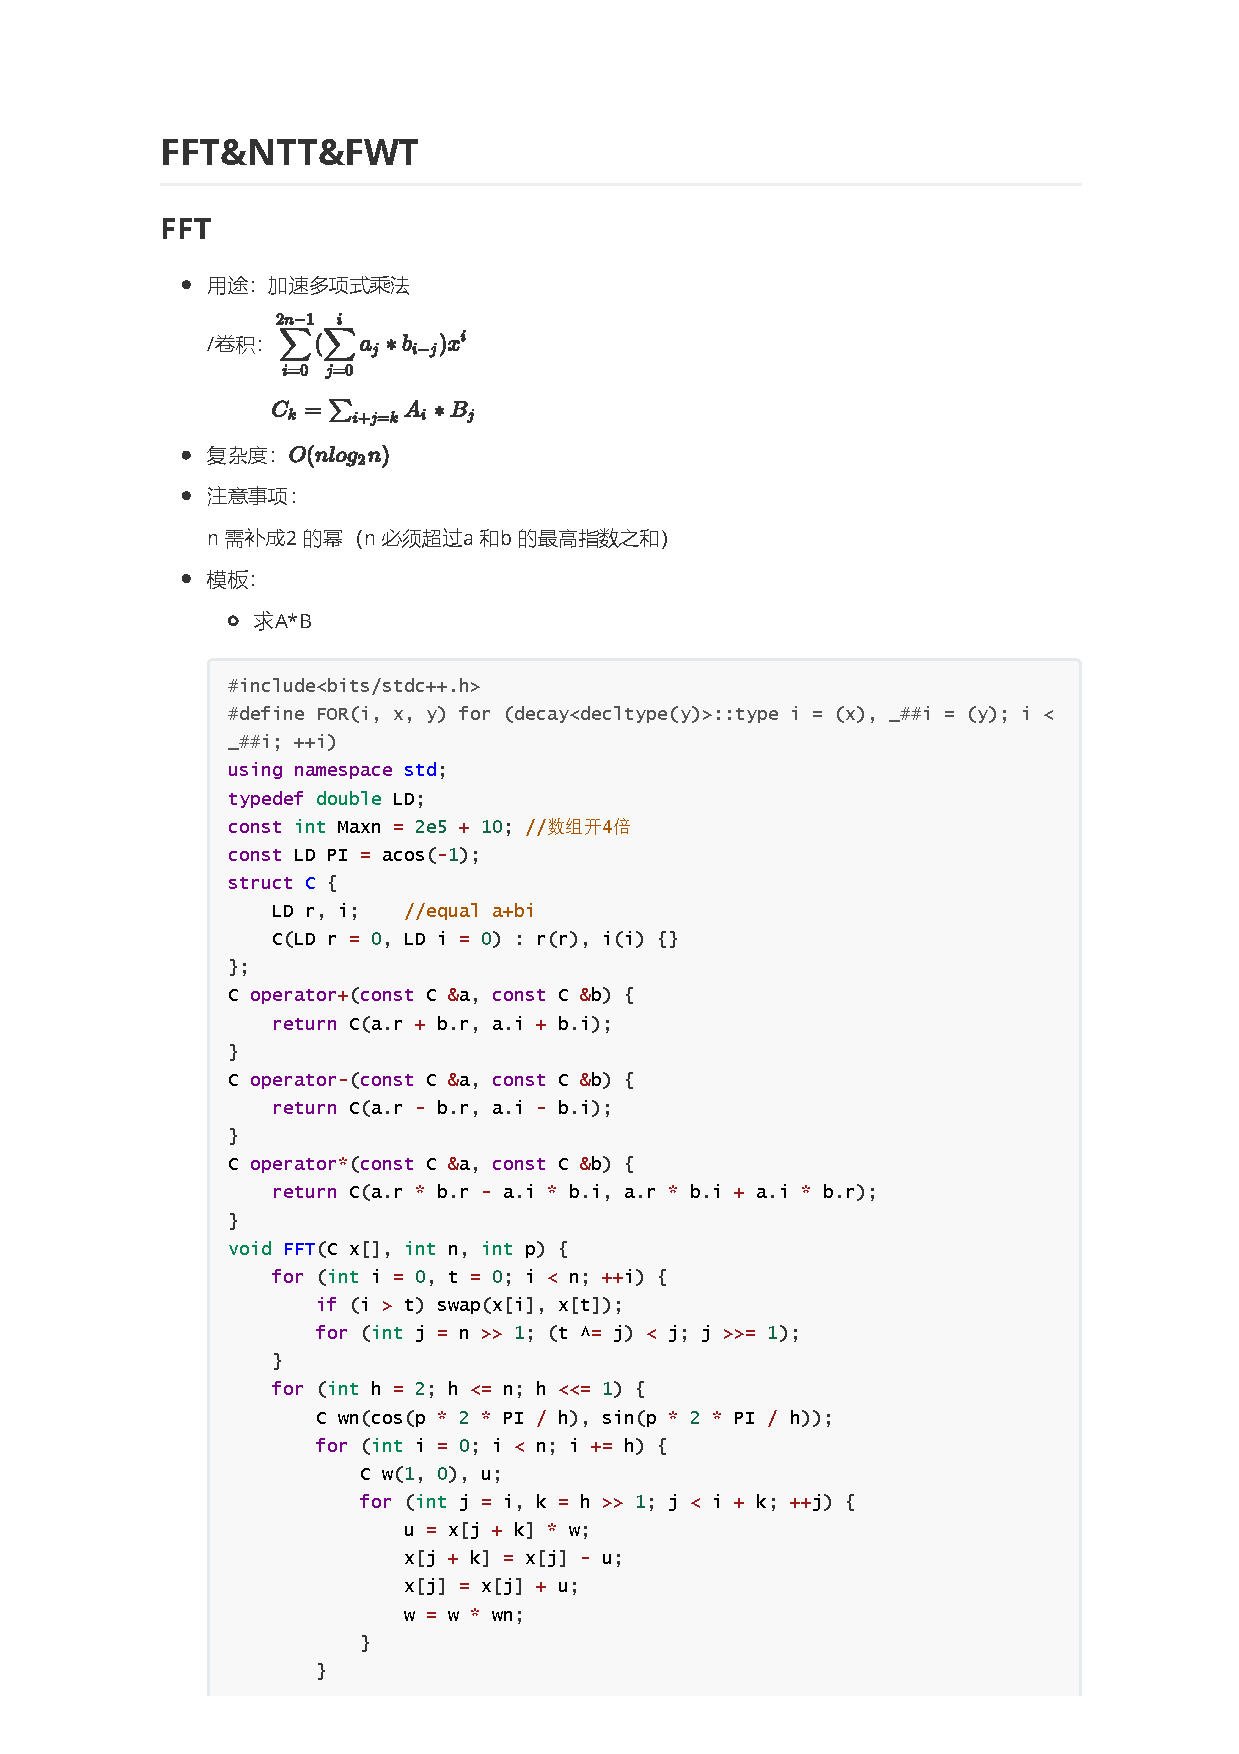
\includepdf[pages={1,2,3,4,5,6}]{Math/FFT&NTT&FWT.pdf}


\newpage
\section{杂项}

\subsection{约瑟夫问题}
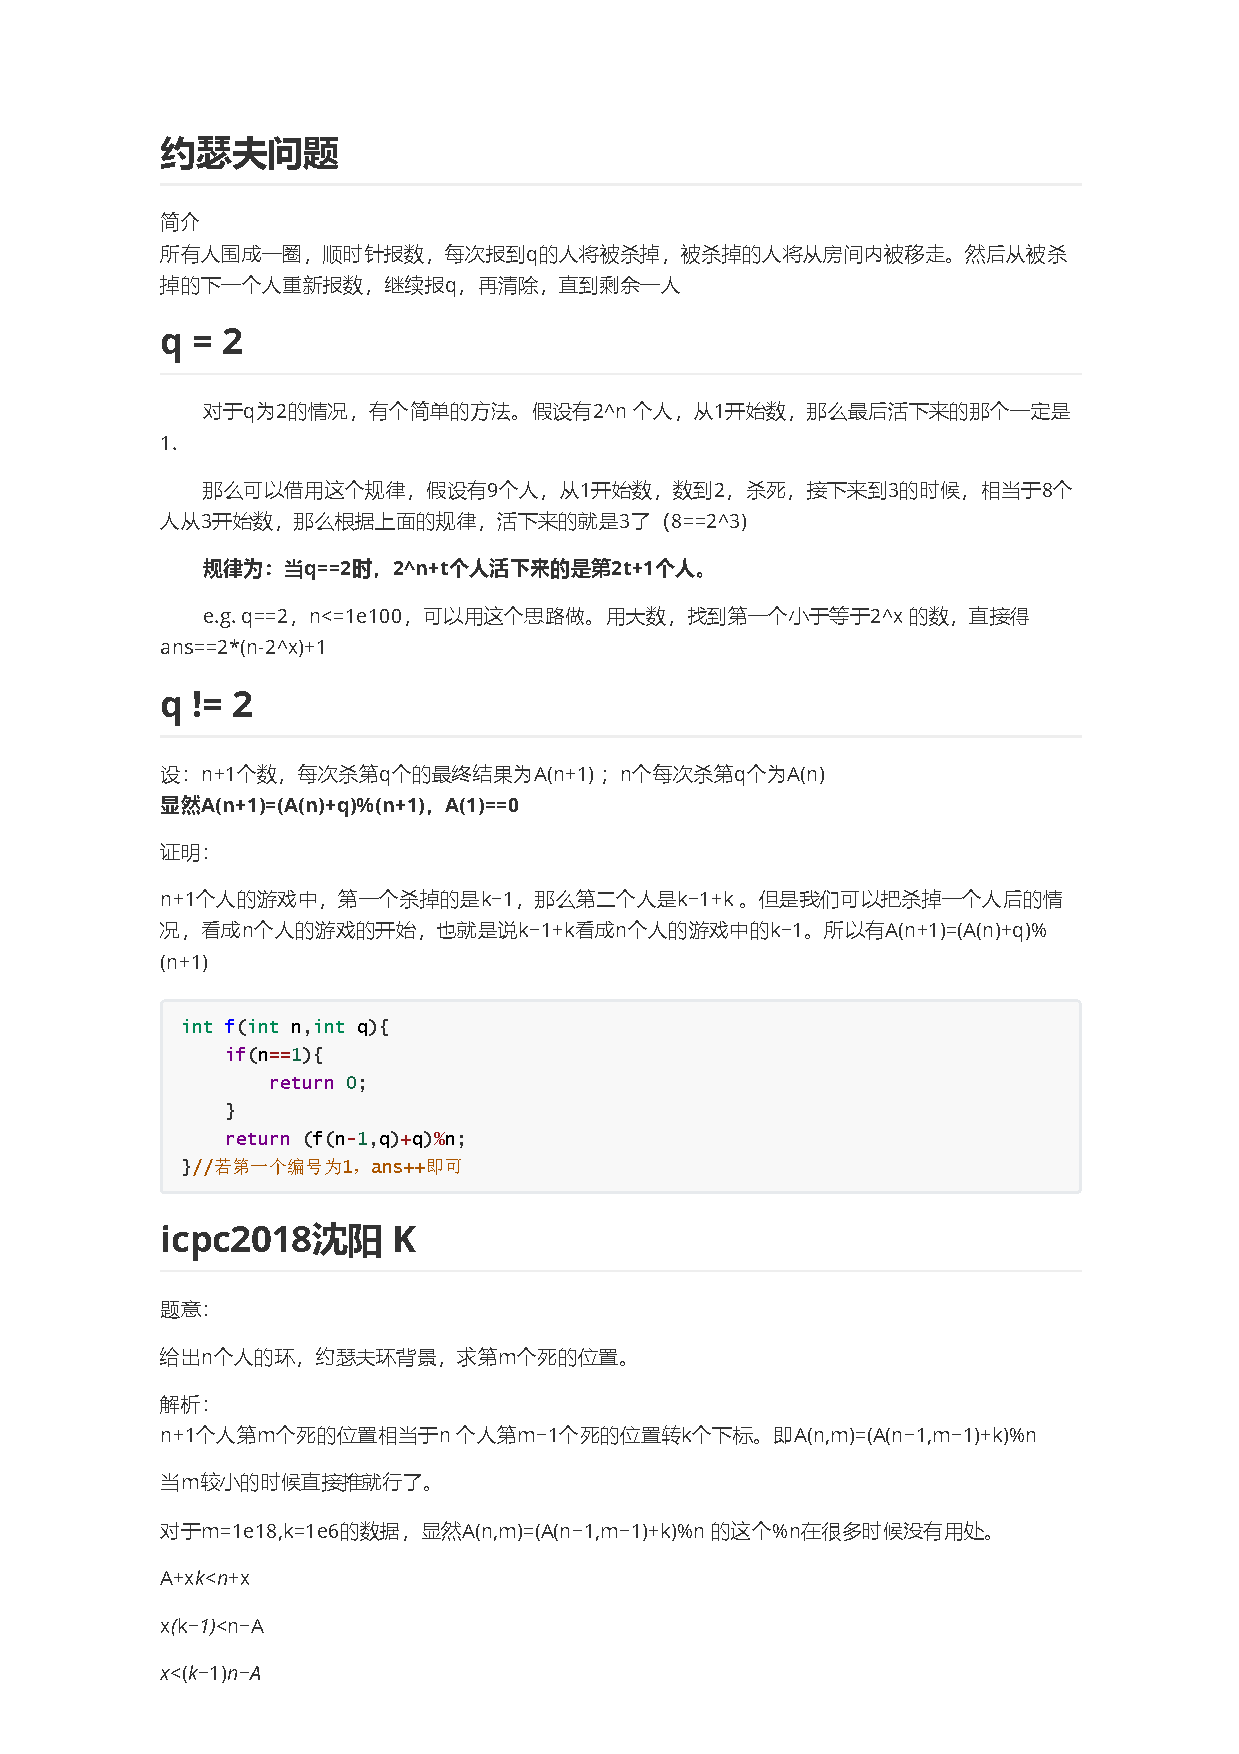
\includepdf[pages={1,2,3}]{Others/约瑟夫问题.pdf}

\subsection{RSA}
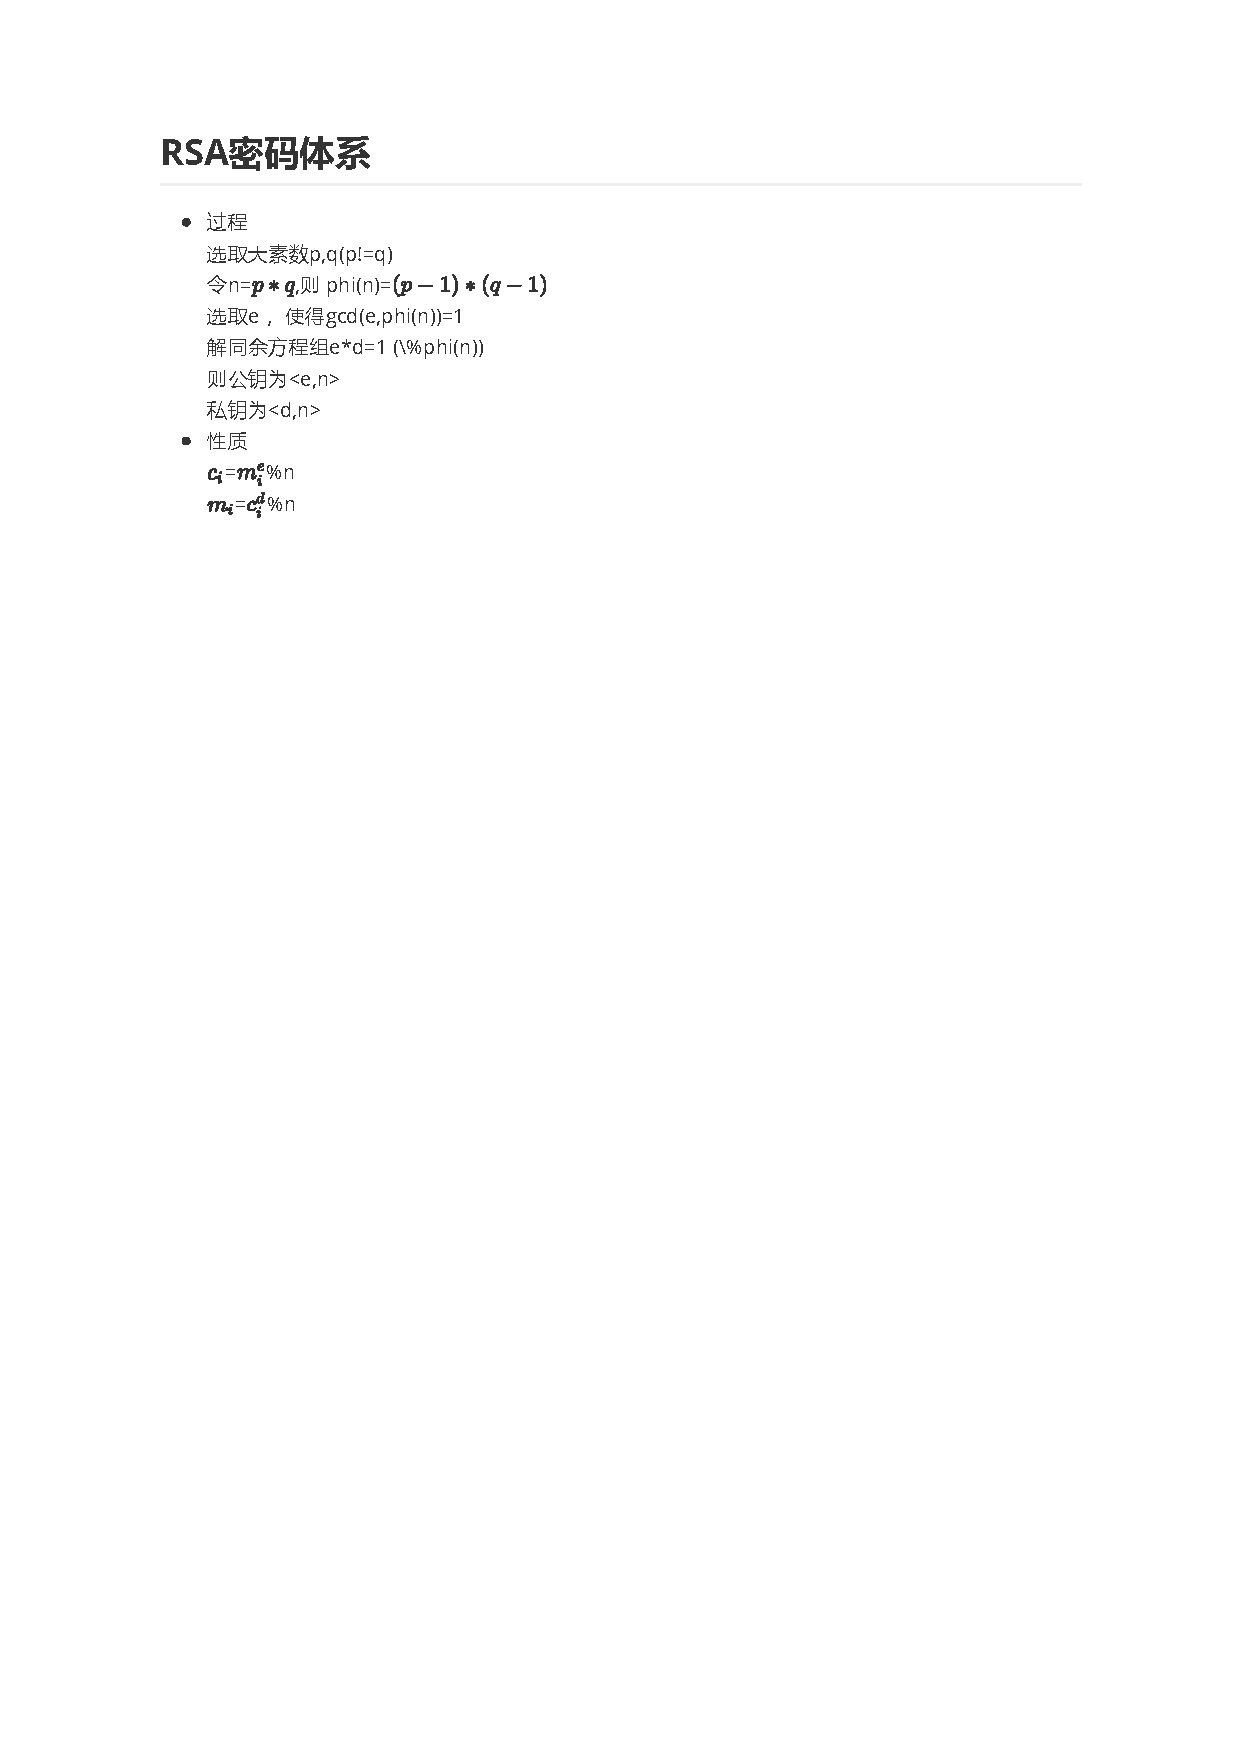
\includepdf[pages={1}]{Others/RSA.pdf}

\subsection{快速读}
\inputminted[breaklines]{c++}{Others/quick_IO.cpp}







\newpage
\section{计算几何}







%\newpage
%\section{Others}

\end{document}


